\documentclass{standalone}

% Fonts
\usepackage[T1]{fontenc}
\usepackage[utf8]{inputenc}
\usepackage{newpxtext,newpxmath}
\usepackage{sectsty}

\usepackage{xcolor}
\usepackage{tikz}
\usetikzlibrary{arrows.meta,calc,positioning}
\usetikzlibrary{shapes.multipart, arrows.meta, positioning, matrix}
\usetikzlibrary{trees}
\usetikzlibrary{trees}
\usepackage{pgfplots}
\pgfplotsset{compat=1.17}
\usepackage{pgfgantt}
% define your status‐styles once
\tikzset{
	notstarted/.style = {circle,draw,fill=gray!20,minimum size=6mm,inner sep=0pt},
	inprogress/.style = {circle,draw,fill=yellow!60,minimum size=6mm,inner sep=0pt},
	done/.style        = {circle,draw,fill=green!60,minimum size=6mm,inner sep=0pt},
	snake it/.style={decorate, decoration=snake},
}

\begin{document}
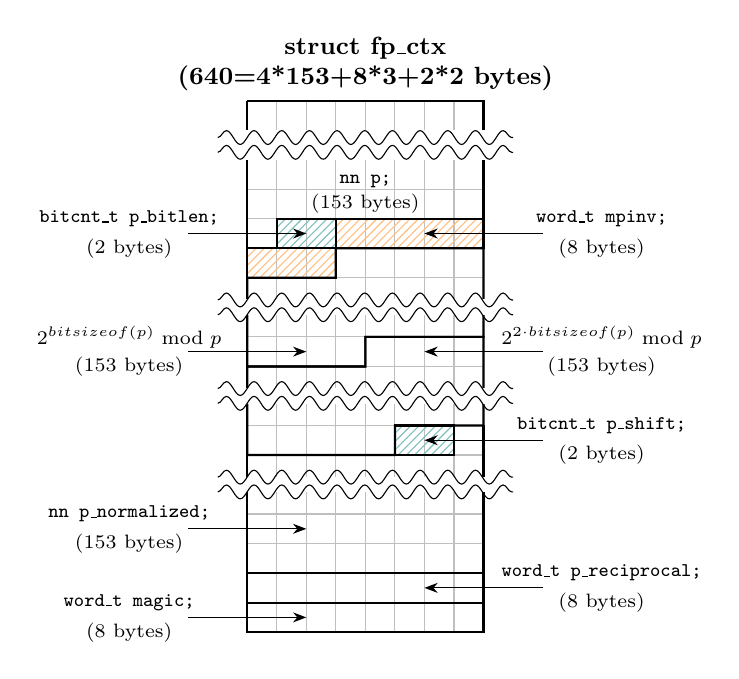
\begin{tikzpicture}[x=1cm, y=-0.05cm, font=\scriptsize, draw=black, >=Stealth, scale=.75]
	\draw[gray!50, step=0.5cm] (0,0) grid (4, 180);
	%		\draw[thick] (0,0) rectangle ++(4,60);  % 128 bytes tall, 3 cm wide
	\draw[thick] (0,0) -- ++(0,50) -- ++(.5,0) -- ++(0,-10) -- ++(3.5,0) -- ++(0,-40) -- ++(-4,0);
	\filldraw[white] (-.5,10) rectangle (4.5, 20);
	\draw[snake it] (-.5,12.5) -- (4.5,12.5);
	\draw[snake it] (-.5,17.5) -- (4.5,17.5);
	% BlockCipherContext labels and offsets
	\node[anchor=south, align=center, font=\small] at (2,0) {\textbf{struct fp\_ctx}\\ \textbf{(640=4*153+8*3+2*2 bytes)}};
	\node[align=center] at (2,27.5) {\texttt{nn p;}};
	\node[align=center] at (2,35) {(153 bytes)};
	\node[align=center] at (-2,40) {\texttt{bitcnt\_t p\_bitlen;}};
	\node[align=center] at (-2,50) {(2 bytes)};
%	\node[align=center, blue] (fp) at (4.5,30) {$\mathbb{F}_p$};
%	\draw[->, blue] (fp) -- ++(-1.5,0);
	\draw[thick, pattern color=teal!50, pattern=north east lines] (.5,50) -- ++(1,0) -- ++(0,-10) -- ++(-1,0) -- cycle;
	\draw[->] (-1,45) -- ++(2,0);
	\draw[thick, pattern color=orange!50, pattern=north east lines] (0,50) -- ++(0,10) -- ++(1.5,0) -- ++(0,-10) -- ++(2.5,0) -- ++(0,-10) -- ++(-2.5,0) -- ++(0,10) -- cycle ;

	\node[align=center] at (6,40) {\texttt{word\_t mpinv;}};
	\node[align=center] at (6,50) {(8 bytes)};
	\draw[->] (5,45) -- ++(-2,0);
	
	\draw[thick] (1.5,60) -- ++(-1.5,0) -- ++(0,30) -- ++(2,0) -- ++(0,-10) -- ++(2,0) -- ++(0,-30) -- ++(-2.5,0) -- cycle;
	\filldraw[white] (-.5,67.5) rectangle (4.5, 72.5);
	\draw[snake it] (-.5,67.5) -- (4.5,67.5);
	\draw[snake it] (-.5,72.5) -- (4.5,72.5);
	
	\node[align=center] at (-2,80) {\texttt{$2^\text{bitsizeof(p)} \bmod p$}};
	\node[align=center] at (-2,90) {(153 bytes)};
	\draw[->] (-1,85) -- ++(2,0);
	
	\draw[thick] (2,90) -- ++(-2,0) -- ++(0,30) -- ++(2.5,0) -- ++(0,-10) -- ++(1.5,0) -- ++(0,-30) -- ++(-2,0) -- cycle;
	\filldraw[white] (-.5,97.5) rectangle (4.5, 102.5);
	\draw[snake it] (-.5,97.5) -- (4.5,97.5);
	\draw[snake it] (-.5,102.5) -- (4.5,102.5);
	
	\node[align=center] at (6,80) {\texttt{$2^{2\cdot\text{bitsizeof(p)}} \bmod p$}};
	\node[align=center] at (6,90) {(153 bytes)};
	\draw[->] (5,85) -- ++(-2,0);
	
	\draw[thick, pattern color=teal!50, pattern=north east lines] (2.5,120) -- ++(1,0) -- ++(0,-10) -- ++(-1,0) -- cycle;
	
	\node[align=center] at (6,110) {\texttt{bitcnt\_t p\_shift;}};
	\node[align=center] at (6,120) {(2 bytes)};
	\draw[->] (5,115) -- ++(-2,0);
	
	\draw[thick] (3.5,120) -- ++(-3.5,0) -- ++(0,40) -- ++(4,0) -- ++(0,-50);
	\filldraw[white] (-.5,127.5) rectangle (4.5, 132.5);
	\draw[snake it] (-.5,127.5) -- (4.5,127.5);
	\draw[snake it] (-.5,132.5) -- (4.5,132.5);
	
	\node[align=center] at (-2,140) {\texttt{nn p\_normalized;}};
	\node[align=center] at (-2,150) {(153 bytes)};
	\draw[->] (-1,145) -- ++(2,0);
	
	\draw[thick] (0,160) rectangle (4, 170);
	
	\node[align=center] at (6,160) {\texttt{word\_t p\_reciprocal;}};
	\node[align=center] at (6,170) {(8 bytes)};
	\draw[->] (5,165) -- ++(-2,0);
	
	\draw[thick] (0,170) rectangle (4, 180);
	
	\node[align=center] at (-2,170) {\texttt{word\_t magic;}};
	\node[align=center] at (-2,180) {(8 bytes)};
	\draw[->] (-1,175) -- ++(2,0);
	
%	\filldraw[white] (-.5,67.5) rectangle (4.5, 72.5);
%	\draw[snake it] (-.5,67.5) -- (4.5,67.5);
%	\draw[snake it] (-.5,72.5) -- (4.5,72.5);
	
%	\draw[gray!50, step=0.5cm] (0,0) grid (4, 200);
%	\node[align=center] at (2,35) {\texttt{word\_t magic;}};
%	\draw[thick, dashed] (0,30) -- ++(4,0);
%	\draw[thick, dashed] (0,40) -- ++(.5,0);
%	\node[align=center] at (2,45) {\texttt{u8 wlen;}};
%	\draw[thick, dashed, -Stealth] (1.2,45) -- ++(-1,0);
	
	
	%		\node[align=center] at (2,68) {\texttt{CipherInternal}\\ (union, 792 bytes)};
	%		
	%		\node[anchor=east] at (0,0) {{\tiny\ttfamily 0x000}};   % top address
	%		\node[anchor=east] at (0,8) {{\tiny\ttfamily 0x008}};
	%		\node[anchor=east] at (0,16) {{\tiny\ttfamily 0x010}};
	%		\node[anchor=east] at (0,24) {{\tiny\ttfamily 0x018}};
	%		\node[anchor=east] at (0,120) {{\tiny\ttfamily 0x318}};
	%		\node[anchor=east] at (0,128) {{\tiny\ttfamily 0x320}};
	%		
	%		% Expand union internal_data: AES, ARIA, LEA internal structures side-by-side
	%		% Base alignment line for union (offset 0x08 in context)
	%		\draw[densely dashed, color=gray!50] (3,8) -- ++(14,0) node[anchor=west]{\tiny\ttfamily 0x008};
	%		\draw[densely dashed, color=gray!50] (3,16) -- ++(14,0) node[anchor=west]{\tiny\ttfamily 0x010};
	%		\draw[densely dashed, color=gray!50] (3,24) -- ++(14,0) node[anchor=west]{\tiny\ttfamily 0x018};
	%		\draw[densely dashed, color=gray!50] (3,45) -- ++(14,0) node[anchor=west]{\tiny\ttfamily 0x108};
	%		\draw[densely dashed, color=gray!50] (3,53) -- ++(14,0) node[anchor=west]{\tiny\ttfamily 0x110};
	%		\draw[densely dashed, color=gray!50] (3,75) -- ++(14,0) node[anchor=west]{\tiny\ttfamily 0x128};
	%		\draw[densely dashed, color=gray!50] (3,83) -- ++(14,0) node[anchor=west]{\tiny\ttfamily 0x130};
	%		\draw[densely dashed, color=gray!50] (3,120) -- ++(14,0) node[anchor=west]{\tiny\ttfamily 0x318};
	%		\draw[densely dashed, color=gray!50] (3,128) -- ++(14,0) node[anchor=west]{\tiny\ttfamily 0x320};
	%		
	%		% AES internal struct (80 bytes used out of 120)
	%		\draw (5,8) rectangle ++(3,120);       % union size tall (for visual alignment)
	%		\draw (5,16) -- ++(3,0);
	%		\draw (5,24) -- ++(3,0);
	%		\draw (5,45) -- ++(3,0);
	%		\draw (5,53) -- ++(3,0);
	%		\node[anchor=south, align=center] at (6.5,8) {\textbf{aes\_internal}\\ \textbf{(8+8+240+8=264 bytes)}};
	%		\node at (6.5,12) {\texttt{size\_t block\_size}};
	%		\node at (6.5,20) {\texttt{size\_t key\_len}};
	%		\node[align=center] at (6.5,36) {\texttt{u32 round\_keys[60]} \\ (240 bytes)};
	%		\node at (6.5,49) {\texttt{int nr}\; (4 bytes)};
	%		\node[color=gray, align=center] at (6.5,90) {\footnotesize (unused\\ \footnotesize 528 bytes)};
	%		\filldraw[gray!70, opacity=.2] (5, 53) rectangle (8, 128);
	%		
	%		\filldraw[teal!70, opacity=.2] (5, 8) rectangle (8, 16);
	%		\filldraw[orange!70, opacity=.2] (5, 16) rectangle (8, 24);
	%		\filldraw[red!70, opacity=.2] (5, 24) rectangle (8, 45);
	%		\filldraw[blue!70, opacity=.2] (5, 45) rectangle (8, 53);
	%		
	%		% ARIA internal struct (same as AES, 80 bytes)
	%		\draw (9,8) rectangle ++(3,120);
	%		\draw (9,16) -- ++(3,0);
	%		\draw (9,24) -- ++(3,0);
	%		\draw (9,75) -- ++(3,0);
	%		\draw (9,83) -- ++(3,0);
	%		\node[anchor=south, align=center] at (10.5,8) {\textbf{aria\_internal}\\ \textbf{(8+8+272+8=296 bytes)}};
	%		\node at (10.5,12) {\texttt{size\_t block\_size}};
	%		\node at (10.5,20) {\texttt{size\_t key\_len}};
	%		\node[align=center] at (10.5,50) {\texttt{u32 round\_keys[68]} \\ (272 bytes)};
	%		\node at (10.5,79) {\texttt{int nr}\; (4 bytes)};
	%		\node[color=gray, align=center] at (10.5,104) {\footnotesize (unused\\ \footnotesize 496 bytes)};
	%		\filldraw[gray!70, opacity=.2] (9, 83) rectangle (12, 128);
	%		
	%		\filldraw[teal!70, opacity=.2] (9, 8) rectangle (12, 16);
	%		\filldraw[orange!70, opacity=.2] (9, 16) rectangle (12, 24);
	%		\filldraw[red!70, opacity=.2] (9, 24) rectangle (12, 75);
	%		\filldraw[blue!70, opacity=.2] (9, 75) rectangle (12, 83);
	%		
	%		% LEA internal struct (116 bytes + 4 bytes padding)
	%		\draw (13,8) rectangle ++(3,120);
	%		\draw (13,16) -- ++(3,0);
	%		\draw (13,24) -- ++(3,0);
	%		\draw (13,120) -- ++(3,0);
	%		\node[anchor=south, align=center] at (14.5,8) {\textbf{lea\_internal}\\ \textbf{(8+8+768+8=792 bytes)}};
	%		\node at (14.5,12) {\texttt{size\_t block\_size}};
	%		\node at (14.5,20) {\texttt{size\_t key\_len}};
	%		\node[align=center] at (14.5,64) {\texttt{u32 round\_keys[192]} \\ (768 bytes)};
	%		\node at (14.5,124) {\texttt{int nr}\; (4 bytes)};
	%		
	%		\filldraw[teal!70, opacity=.2] (13, 8) rectangle (16, 16);
	%		\filldraw[orange!70, opacity=.2] (13, 16) rectangle (16, 24);
	%		\filldraw[red!70, opacity=.2] (13, 24) rectangle (16, 120);
	%		\filldraw[blue!70, opacity=.2] (13, 120) rectangle (16, 128);
	%		
	%		% Brace to indicate union grouping
	%		\draw[decorate,decoration={brace,amplitude=4pt}] (16,130) -- node[below=4pt]{Union members (share same memory)} (5,130);
	%		
	%		% BlockCipherApi vtable structure (40 bytes)
	%		% Place vtable below (starting at y=140 for offset 0)
	%		\filldraw[blue!50, opacity=.8] (0, 160) rectangle (3, 168);
	%		\draw[thick] (0,160) rectangle ++(3,32);
	%		\draw[thick] (0,168) -- ++(3,0);
	%		\draw[thick] (0,176) -- ++(3,0);
	%		\draw[thick] (0,184) -- ++(3,0);
	%		%	\draw[thick] (0,192) -- ++(3,0);
	%		\node[anchor=south,align=center] at (1.5,160) {\textbf{BlockCipherApi (vtable)}\\ \textbf{8$\times$4=32 bytes}};
	%		\node at (1.5,164) {\texttt{const char* name}};
	%		\node at (1.5,172) {\texttt{void*}};
	%		\node at (1.5,180) {\texttt{void*}};
	%		%	\node at (1.5,188) {\texttt{void*}};
	%		\node at (1.5,188) {\texttt{void*}};
	%		
	%		% Arrows: BlockCipherContext.api -> vtable, and vtable function ptrs -> functions
	%		% API pointer arrow (from BCC.api field to vtable)
	%		\draw[->, thick] (0,4) -| (-1,4) -- (-1,164) -- ++(1,0);
	%		
	%		% Function implementation nodes for AES
	%		\node[draw, anchor=west, fill=magenta!10] (fn_init)        at (5,172) {\texttt{aes\_init(BlockCipherContext* ctx, /* ... */ );}};
	%		\node[draw, anchor=west, fill=green!10] (fn_encrypt)     at (5,180) {\texttt{aes\_process\_block(BlockCipherContext* ctx, /* ... */ );}};
	%		%	\node[draw, anchor=west, fill=lime!10] (fn_decrypt)     at (3.5,188) {\texttt{decrypt(BlockCipherContext* ctx, const u8* ct, u8* pt);}};
	%		\node[draw, anchor=west, fill=cyan!10] (fn_dispose)     at (5,188) {\texttt{dispose(BlockCipherContext* ctx);}};
	%		
	%		\draw[->] (3,172) -- (fn_init.west);
	%		\draw[->] (3,180) -- (fn_encrypt.west);
	%		%	\draw[->] (3,188) -- (fn_decrypt.west);
	%		\draw[->] (3,188) -- (fn_dispose.west);
\end{tikzpicture}
\end{document}